%%%%%%%%%%%%%%%%%%%%%%%%%%%%%%%%%%%%%%%%%%%%%%%%%%%%%%%%%%%%%%%%%%%%%%%%%%%
%                                                                         %
% Beamer template for slideshow presentations, primarily intended for     %
% University of Milano Bicocca and INFN Bicocca affiliation.              %
% This is based on the 'Università di Siena' template by Barbara Toniella %
% Corradini available on Overleaf. Many corrections and fixes were added  %
% by Matteo Saccardi                                                      %
%                                                                         %
% Pietro Rescigno @ Unimib                                                %
%                                                                         %
%%%%%%%%%%%%%%%%%%%%%%%%%%%%%%%%%%%%%%%%%%%%%%%%%%%%%%%%%%%%%%%%%%%%%%%%%%%

\documentclass[ 11pt, english, xcolor=dvipsnames, aspectratio=43,showframe=true]{beamer}
%\usefonttheme{serif}
% Text encoding
\usepackage[english]{babel}
\usepackage{physics}
\usepackage{amsmath}
\usepackage{dsfont}
\usepackage{footbib}
\usepackage{hyperref}
\usepackage{appendixnumberbeamer}
\usepackage[dvipsnames]{xcolor}
\usepackage{bm}
\usepackage{makecell}
% Justify text (package and function)
% \apptocmd{command}{code}{success}{failure}
\usepackage{ragged2e}
\usepackage{dirtytalk}
\apptocmd{\frame}{}{\justifying}{} 
% Justify text in \item
\newcommand{\itemj}{\item \justifying}
\useinnertheme{circles}
% If...else package
\usepackage{ifthen}

% Package to set transparent background image
\usepackage{tikz}

% Include image package
\usepackage{graphicx}
% Set default path for images
\graphicspath{ {./images/} }
% Set figure number when included
\setbeamertemplate{caption}[numbered]
\newcommand{\Qquad}{\hspace{0.25em}} 
% Bibliography packages
\usepackage[style=authoryear,backend=bibtex]{biblatex}
%\setbeamertemplate{bibliography item}{\insertbiblabel} 
\addbibresource{sample.bib}
%\bibliographystyle{plainnat}
\usepackage[absolute,overlay]{textpos}
% Define colors variables
\definecolor{red}{rgb}{0.631, 0.094, 0.094} % primary color
\definecolor{grey}{HTML}{708090} % secondary color
\definecolor{blue}{rgb}{0,0,0.54}
\definecolor{dgrey}{HTML}{1F3B4D}
% Set theme palette colors
\setbeamercolor{palette primary}{bg=red,fg=white}
\setbeamercolor{palette secondary}{bg=red,fg=white}
\setbeamercolor{palette tertiary}{bg=red,fg=white}
\setbeamercolor{palette quaternary}{bg=red,fg=white}
% strucure means itemize, enumerate, etc
\setbeamercolor{structure}{fg=red} 

\setbeamercolor{alerted text}{fg = red}

% Set bibliography colors
\setbeamercolor{bibliography item}{fg=red}
\setbeamercolor{bibliography entry author}{fg=black}
\setbeamercolor{bibliography entry title}{fg=black}
\setbeamercolor{bibliography entry location}{fg=black}
\setbeamercolor{bibliography entry note}{fg=black}
% Replaces book icon in bibliography with enumeration
%\setbeamertemplate{bibliography item}{[\theenumiv]}

% Table of contents style
% \setbeamertemplate{section in toc}[sections numbered]
% \setbeamertemplate{subsection in toc}[subsections numbered]
\setbeamertemplate{section in toc}[circle]
\setbeamertemplate{subsection in toc}[ball unnumbered]

\setbeamertemplate{navigation symbols}{}

% Header with navigation bar
\setbeamertemplate{headline}
{
    
    \ifnum \theframenumber=1  % Title frame 
        %title frame:nothing  % without headline
    \else
      \setbeamerfont{section in head/foot}{size=\small}
      \leavevmode
      \hbox{
      \begin{beamercolorbox}[wd=\paperwidth,ht=6ex,dp=3ex]{palette primary}
        \insertsectionnavigationhorizontal{\paperwidth}{}{}
      \end{beamercolorbox} 
      }
    \fi
}

% Footer with custom caption
\setbeamertemplate{footline}
{
    \ifnum \theframenumber=1    % Title Frame
        %title frame: nothing   % without footline
    \else
        \leavevmode
        \hbox{
        \begin{beamercolorbox}[wd=.23\paperwidth,ht=2.6ex,dp=1ex,center]{palette primary}
            \usebeamerfont{author in head/foot}\insertshortauthor\hspace*{1ex}
        \end{beamercolorbox}
        \begin{beamercolorbox}[wd=.53\paperwidth,ht=2.6ex,dp=1ex,center]{palette secondary}
            \usebeamerfont{title in head/foot}\insertshorttitle
        \end{beamercolorbox}
        \begin{beamercolorbox}[wd=.23\paperwidth,ht=2.6ex,dp=1ex,center]{palette quaternary}
            \insertframenumber{} / \inserttotalframenumber
        \end{beamercolorbox}}
        \vskip0pt
    \fi
}

% One line command to print table of contents - two parameters for modes
\newcommand{\customToC}[2]
{
    \begin{frame}{Overview}
    \tableofcontents[#1,#2]
    \end{frame}
}

% Command to plot centered figure
% Parameters: #1=image name, #2=caption 
\newcommand{\includefigure}[2]
{
    \begin{figure}[h]
    \caption{#2}
    \centering
    \includegraphics[width=0.5\textwidth]{#1}
    \end{figure}
}

% Command to set section name as variable (\renewcommand to update)
\newcommand{\sectiontitle}{}
% Command to set subsection name as variable (\renewcommand to update)
\newcommand{\subsectiontitle}{}

\setbeamertemplate{blocks}[default]

% This will go in the footline
\title{Title of the presentation}
\author{Pietro Rescigno}
\institute{Università degli studi di Milano-Bicocca}
% Date
\day=23\relax
\month=11\relax
\year=2022\relax

\begin{document}

% GLOBAL background must be put in preamble
% This produces a centered background that fills up the page on EVERY SLIDE
% To set background to specific frames (eg title only), enclose this command in { } around the slide

%\setbeamertemplate{background canvas}{

%        \tikz[remember picture,overlay] {\node[inner sep=0pt,opacity=0.3] at (current page.center)
%        {\includegraphics[height=\paperheight,width=\paperwidth]{Background/bicooca_background.png}};}

%}


%%%%%%%%%%%%%%%%%%%%%%%%%%%%%%%%%%%%%%%%%%%%%%%%%%%%%%%
% "Lattice Lunch" title page
%%%%%%%%%%%%%%%%%%%%%%%%%%%%%%%%%%%%%%%%%%%%%%%%%%%%%%%
%\begin{frame}{}
%        \large{\color{red}\textbf{Lattice Lunch Seminars}} \hfill \normalsize{Date, Pietro Rescigno}\vspace{1mm}\hrule\\[6mm]
        
%        {\large{\textbf{Title here}}}\\[6mm]
        
%        \textit{Authors / subtitle here} \\[4mm]
        
%        Journal name\\
%        \href{}{arXiv: }\\
%        Published gg-mm-yyyy
%
%        % Logos here
%        \begin{textblock*}{5cm}(9.45cm,6.8cm)
%            \includegraphics[scale=0.7]{logos/logo_unimib.pdf}
%        \end{textblock*}
%        \begin{textblock*}{5cm}(11.45cm,6.8cm)
%            
\includegraphics[scale=0.15]{logos/1_MILANOB_LOGO_SIGLA.pdf}
%        \end{textblock*}
%\end{frame}
%%%%%%%%%%%%%%%%%%%%%%%%%%%%%%%%%%%%%%%%%%%%%%%%%%%%%%%

%%%%%%%%%%%%%%%%%%%%%%%%%%%%%%%%%%%%%%%%%%%%%%%%%%%%%%%
% Seminar / Talk title page
%%%%%%%%%%%%%%%%%%%%%%%%%%%%%%%%%%%%%%%%%%%%%%%%%%%%%%%

{ % This is to set local background
    % Bicocca background has 1:1 proportion
    \usebackgroundtemplate{\tikz[remember picture,overlay] {\node[inner sep=0pt,opacity=0.2] at (current page.center)
        {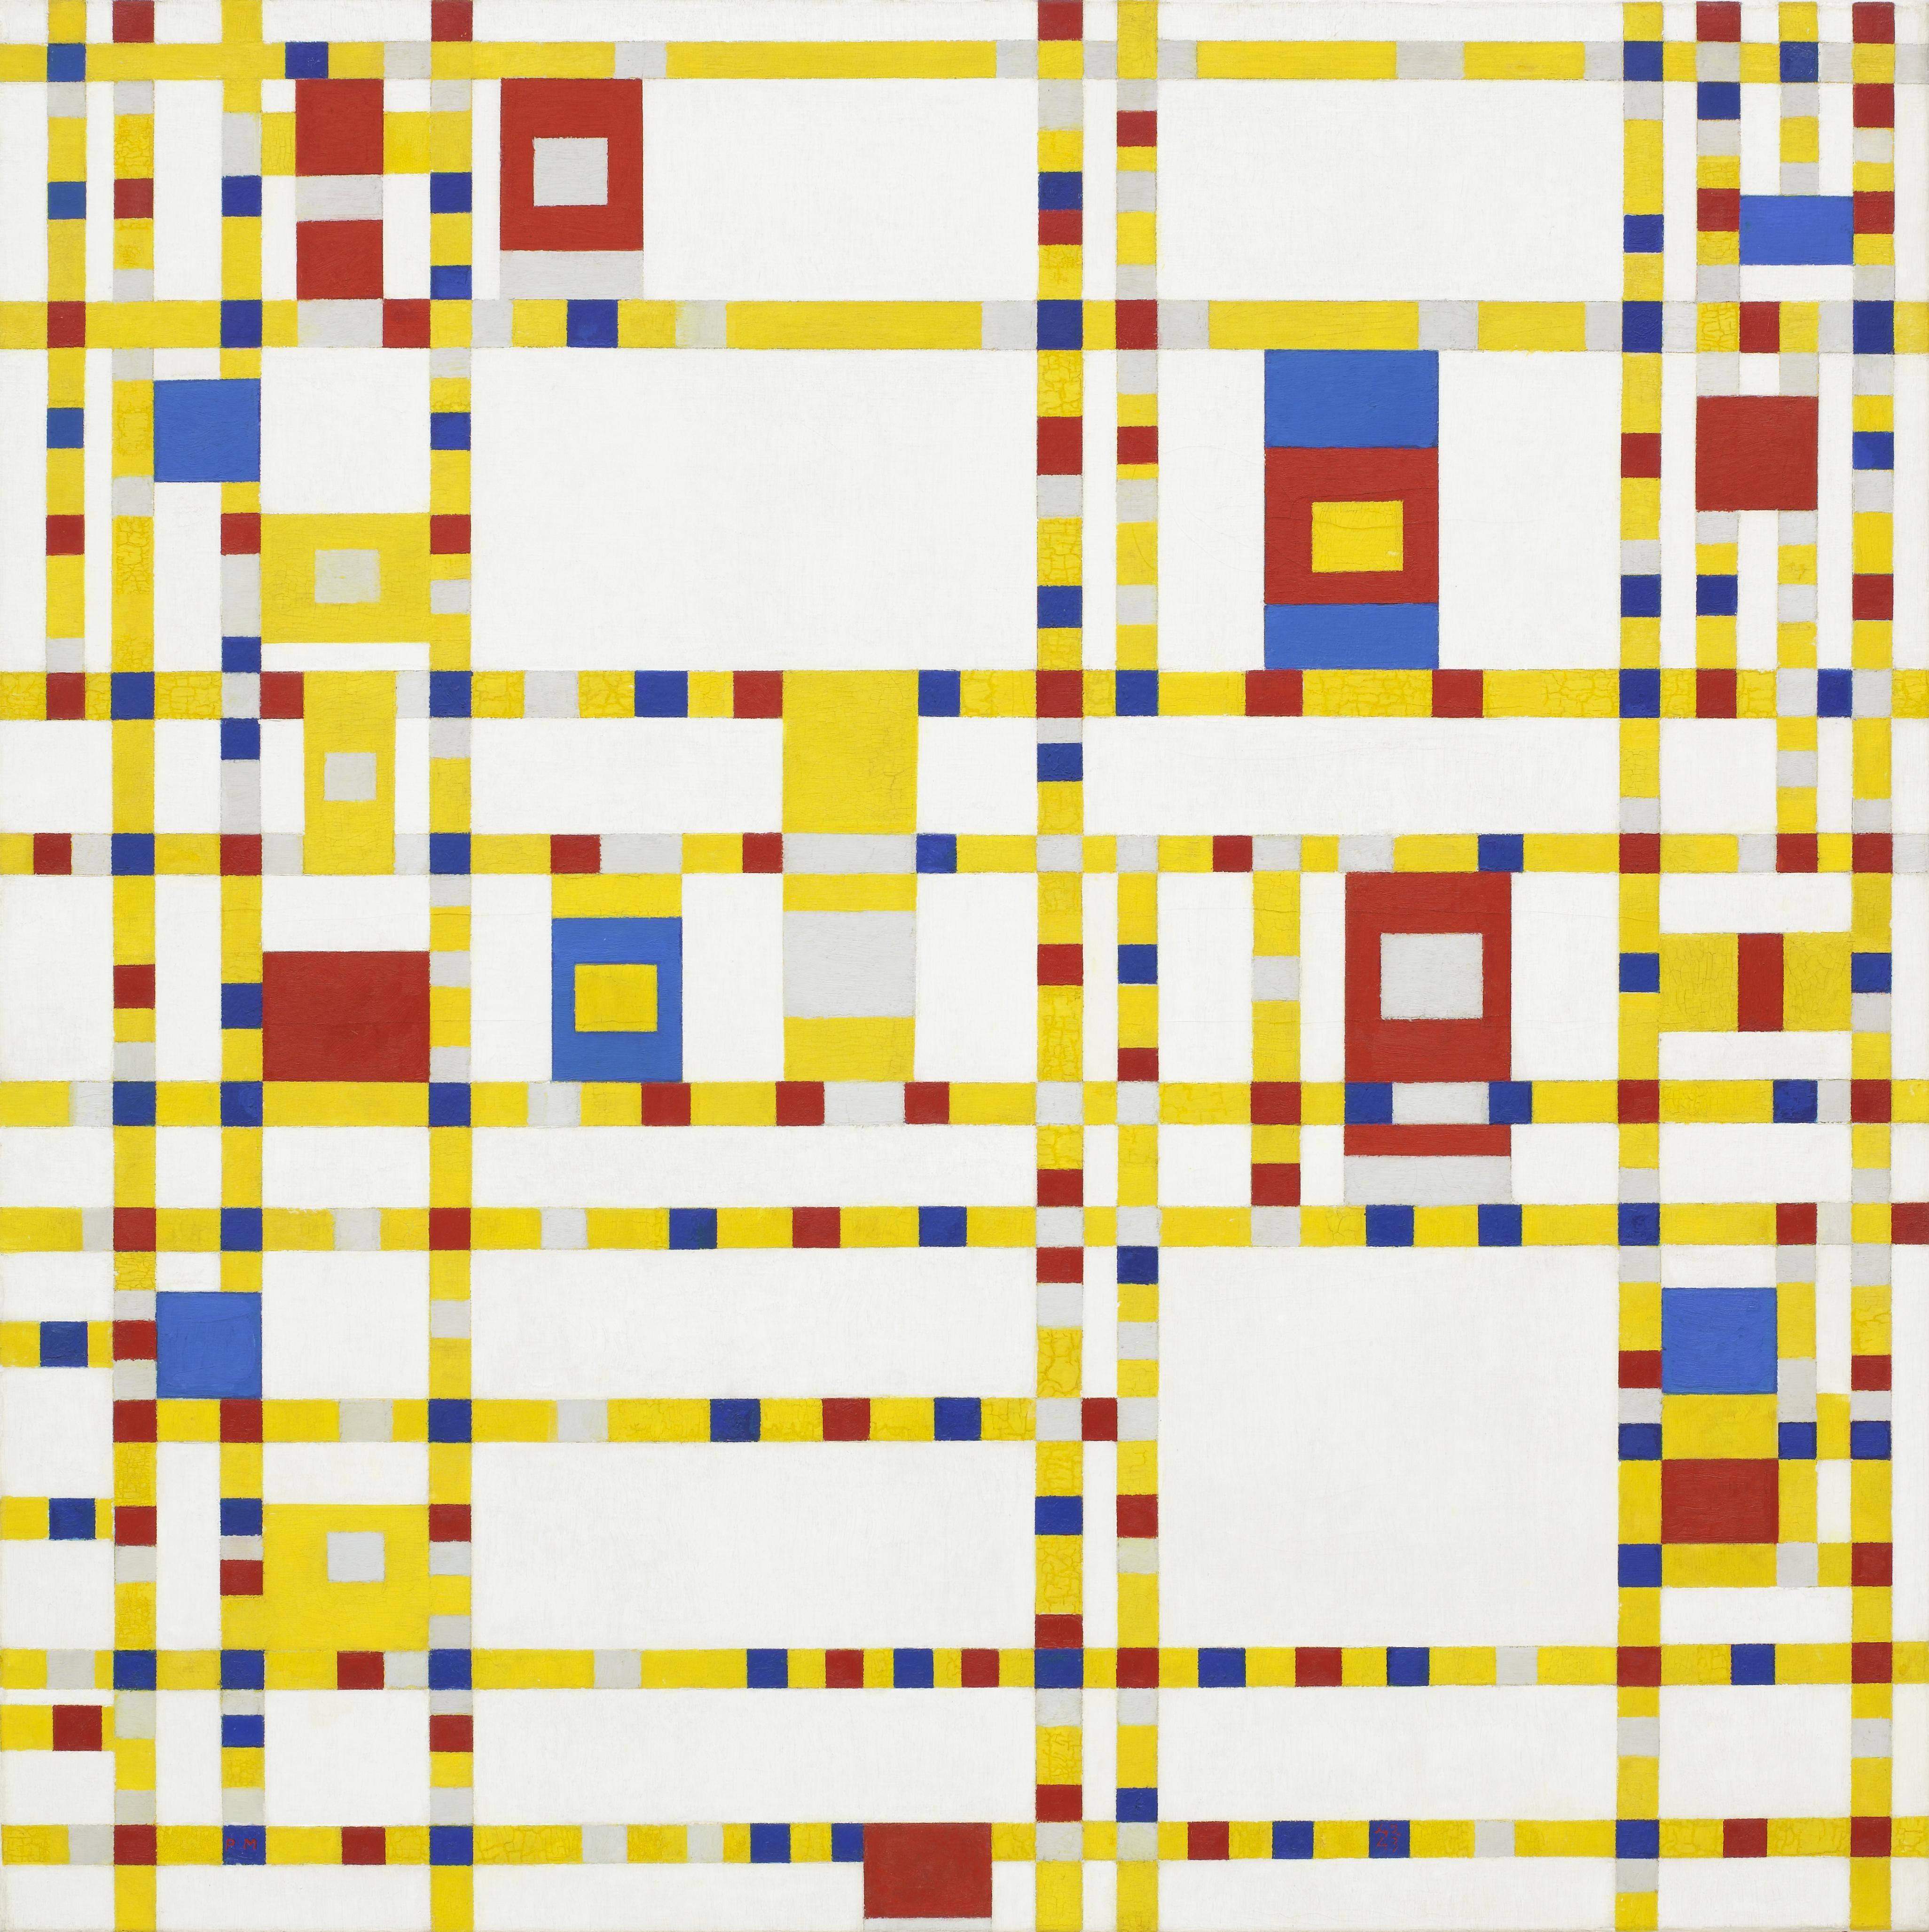
\includegraphics[height=\paperheight,width=\paperwidth]{Background/Mondrian.jpg}};}}
    \begin{frame}{}
        \vspace{-1.2cm}
        {\centering
        {\huge\textbf{\alert{Title here}}}\\[2mm]
        {\textbf{Speaker}}$^{a,b}$\\[2mm]}
        \hline\\[2mm]
        Tizio$^{\textit{a},b}$, Caio$^{a,b}$, Sempronio$^{c}$\\[3mm]
        \hspace{\hskip} \textit{$^a$ U.S. Robots and Mechanical Men, Inc.}\\
        \hspace{\parindent} \textit{$^b$ Aperture Science Enrichment Centre}\\
        \hspace{\parindent} \textit{$^c$ Black Mesa}\\

        %% Logos go here %%
        \begin{textblock*}{5cm}(1.1cm,6.55cm)
            
\includegraphics[scale=0.025]{logos/Bicocca_transparent.png}
        \end{textblock*}
        \begin{textblock*}{5cm}(2.4cm,6.6cm)
            
\includegraphics[scale=0.15]{logos/1_MILANOB_LOGO_SIGLA.pdf}
        \end{textblock*}
        % Extra logos (Conference)
        %\begin{textblock*}{5cm}(8.2cm,6.9cm)
        %        \includegraphics[scale=0.15]{logos/Lattice23logo.png}
        %\end{textblock*}
        

    \end{frame}
} % Close background bracket

\section{Section 1}
\begin{frame}{}

    \begin{itemize}
        \item Some text
        \item Some text
        \item more text
    \end{itemize}
\end{frame}

\section{Section 2}

\begin{frame}{}

        \begin{itemize}
        \item Some text
        \item Some text
        \item more text
    \end{itemize}
        
\end{frame}


\section{Conclusions}
\begin{frame}{}
    \begin{itemize}
        \item Some text
        \item Some text
        \item more text
    \end{itemize}
\end{frame}

\newcounter{totalmainframes}
\setcounter{totalmainframes}{\value{framenumber}}
\appendix
\section{Backup}
\begin{frame}{}
	\Large{\texbf{\centering{Back Up}}}
\end{frame}
\begin{frame}{}

	Backup slides
\end{frame}
\end{document}
